      
               
                \begin{ledgroupsized}[r]{120mm}
                \footnotesize 
                \pstart                
                \noindent\textbf{\"{U}berlieferung:}   
                \pend
                \end{ledgroupsized}
            
              
                            \begin{ledgroupsized}[r]{114mm}
                            \footnotesize 
                            \pstart \parindent -6mm
                            \makebox[6mm][l]{\textit{L}}Exzerpte: LH XXXV 14, 2 Bl. 91\textendash102. 6 Bog. 2\textsuperscript{o}. 11 S. zweispaltig. Textfolge: Bl. 95 v\textsuperscript{o}, 99 v\textsuperscript{o}, 94 r\textsuperscript{o}, 97 v\textsuperscript{o}, 96 r\textsuperscript{o}, 98 r\textsuperscript{o}, 101 v\textsuperscript{o}, 100 r\textsuperscript{o}, 93 v\textsuperscript{o}, 92 r\textsuperscript{o}, 91~v\textsuperscript{o}. Zeichnungen auf Bl. 92 r\textsuperscript{o}, 94 r\textsuperscript{o}, 95 v\textsuperscript{o}, 96 r\textsuperscript{o} und 99 v\textsuperscript{o}. Auf Bl. 91 v\textsuperscript{o} umfangreichere Rechnungen. Die folgenden Seiten leer: Bl. 91 r\textsuperscript{o}, 92 v\textsuperscript{o}, 93 r\textsuperscript{o}, 94 v\textsuperscript{o}, 95 r\textsuperscript{o}, 96 v\textsuperscript{o}, 97 r\textsuperscript{o}, 98 v\textsuperscript{o}, 99 r\textsuperscript{o}, 100 v\textsuperscript{o}, 101 r\textsuperscript{o} und 102 r\textsuperscript{o}, v\textsuperscript{o}.\\
 Cc 2, Nr. 474 A, B \pend
                            \end{ledgroupsized}
                %\normalsize
                \vspace*{5mm}
                \begin{ledgroup}
                \footnotesize 
                \pstart
            \noindent\footnotesize{\textbf{Datierungsgr\"{u}nde}: Otto von Guerickes \cite{00055}\textit{Experimenta nova} wurden im Mai 1672 ausgeliefert. Darin enthaltene neue Experimente und Beobachtungen wurden von Leibniz erstmals in Texten erw\"{a}hnt, die in der Zeit zwischen dem 25. Juli und dem 12. Dezember 1672 entstanden sind. Leibniz muss die \cite{00055}\textit{Experimenta nova} also bereits vorher gekannt haben. Wir datieren die Entstehungszeit dieser Exzerpte daher auf den Sommer 1672.}
                \pend
                \end{ledgroup}
            
                \vspace*{8mm}
                \pstart 
                \normalsize
            [95 v\textsuperscript{o}] \edtext{Schottus\protect\index{Namensregister}{\textso{Schott} (Schottus), Caspar SJ 1608\textendash 1666} Experimenta Magdeburgica\protect\index{Sachverzeichnis}{experimentum!Magdeburgicum} bis descripsit  primum in arte \edtext{\textit{Hydraulico-pneumatica},}{\lemma{\textit{Hydraulico-pneumatica}}\Bfootnote{\textsc{C. Schott, }\cite{00095}\textit{Mechanica hydraulico-pneumatica}, Frankfurt 1657, S.~441\textendash484.%\protect\hspace{30pt}
            }} deinde in \edtext{\textit{Technica}}{\lemma{\textit{Technica}}\Bfootnote{\textsc{C. Schott, }\cite{00096}\textit{Technica curiosa}, N\"{u}rnberg 1664, 1. Buch.}}.}{\lemma{}\Afootnote{Schottus\protect\index{Namensregister}{\textso{Schott} (Schottus), Caspar SJ 1608\textendash 1666} Experimenta Magdeburgica\protect\index{Sachverzeichnis}{experimentum!Magdeburgicum} bis descripsit  primum in arte \textit{Hydraulico-pneumatica}, deinde in \textit{Technica}. \textit{ erg.} \textit{ L}}} Otto Gerickii\protect\index{Namensregister}{\textso{Guericke} (Gerickius, Gerick.), Otto v. 1602\textendash 1686} \cite{00055}\textit{Experimenta nova ut vocantur Magdeburgica de spatio vacuo} Amst.\protect\index{Ortsregister}{Amsterdam} ap. Joh. Janson de Waesberge\protect\index{Namensregister}{\textso{Waesberge,} Johannes Jansson zu 1651\textendash 1681} 1672. fol.\pend 
            \newpage
            \pstart \textso{Gerick. lib. 1.} c. 19.\edtext{}{\lemma{19.}\Bfootnote{\textsc{O. v. Guericke, }\cite{00055}\textit{Experimenta nova}, Amsterdam 1672, S.~26. }} citat Hevelii\protect\index{Namensregister}{\textso{Hevelius,} Johannes 1611\textendash 1687} \textit{diss. de nativa Saturni facie ejusque variis phasibus certa periodo redeuntibus},\edtext{}{\lemma{\textit{redeuntibus},}\Bfootnote{\textsc{J. Hevelius, }\cite{00059}\textit{Dissertatio de nativa saturni facie}, Danzig 1656.}} et Christ. Hugenii\protect\index{Namensregister}{\textso{Huygens} (Hugenius, Vgenius, Hugens, Huguens), Christiaan 1629\textendash 1695} lib. pecul. 1659.  de \textit{Systemate Saturnio}.\edtext{}{\lemma{\textit{Saturnio}.}\Bfootnote{\textsc{Chr. Huygens, }\cite{00065}\textit{Systema Saturnium}, Den Haag 1659. }} Hevelii\protect\index{Namensregister}{\textso{Hevelius,} Johannes 1611\textendash 1687} liber ni fallor  fuit prior, et Hugenio\protect\index{Namensregister}{\textso{Huygens} (Hugenius, Vgenius, Hugens, Huguens), Christiaan 1629\textendash 1695} facem alluxit.\pend \pstart \textso{C. 35.}\edtext{}{\lemma{\textso{35.}}\Bfootnote{\textsc{O. v. Guericke}, \cite{00055}a.a.O., S.~52.}} refert Lessium\protect\index{Namensregister}{\textso{Lessius,} L\'{e}onard 1554\textendash 1623} \textit{perfect. divin.}  lib. 2. cap. 2.\edtext{}{\lemma{2.}\Bfootnote{\textsc{L. Lessius, }\cite{00070}\textit{De perfectionibus}, Antwerpen 1624, S.~27.}} statuentem, spatium infinitum imaginarium, esse ipsum DEUM, (+ Timplerus\protect\index{Namensregister}{\textso{Timpler} (Timplerus), Clemens 1567\textendash 1624} quoque DEUM esse locum coeli +)  et ipse cap. 6. lib. 2.\edtext{}{\lemma{2.}\Bfootnote{\textsc{O. v. Guericke}, \cite{00055}a.a.O., S.~60.}} idem innuere  videtur Gerickius\protect\index{Namensregister}{\textso{Guericke} (Gerickius, Gerick.), Otto v. 1602\textendash 1686} etsi enuntiare satis clare non audeat  et clarius cap. 9.\edtext{}{\lemma{9.}\Bfootnote{\textsc{O. v. Guericke}, \cite{00055}a.a.O., S.~64f.}} spatium rerum esse ipsam divinam essentiam tam intra quam extra Mundum\protect\index{Sachverzeichnis}{mundus}.\pend \pstart \textso{Lib. 2. c. 10.}\edtext{}{\lemma{\textso{10.}}\Bfootnote{\textsc{O. v. Guericke}, \cite{00055}a.a.O., S.~67f.}} \textit{per interrogationem simulque  sponsionem detuli 100 thaleros cuidam Arithmetico excellenti pro labore ejus si intra destinatum tempus quartam scilicet anni partem, quo  inter nos conventum fuerat computare posset  summam Numeri 2. vicies }\edtext{\textit{quadratice}}{\lemma{}\Afootnote{\textit{quadratice} \textit{ erg.} \textit{ L}}}\textit{ in se ducti.} \textit{Ille promittebat deponens 10 imperiales, et quidem non  intra anni quadrantem sed unum mensem se praestiturum illud, et productum propositi exempli elapso tempore in praesentia eorum qui tunc aderant  adhibere, non cogitans ob emergentem characterum multitudinem, id opus nullius esse mortalis,  ut sequitur in operatione:} \pend 
            \pstart \textit{2. semel in se ducta faciunt 4}\pend
            \pstart \textit{2 bis (id est 4.) in se ducta faciunt 16.} \pend
            \pstart \textit{2 ter in se ducta (id est} $2^\smallfrown 2 = 4.^\smallfrown 4 = 16.^\smallfrown 16. =  256$\textit{)} \pend 
            \pstart \textit{2 quater (id est 256) in se ducta faciunt 65536.} \pend
            \pstart \textit{2. quinquies in se ducta faciunt 4294967  296.} \pend 
            \pstart \textit{2 sexies in se ducta faciunt 18446744073 }\textit{ 709551616; etc.} \pend 
            \pstart Ex his videmus tali modo si semper productus rursus  in se ducatur; et ita procedatur vicies  duplum fere semper oriri numerum characterum. Ergo in septima multiplicatione  fierent cyphrae 40, in octava 80, in  vigesima Zyphrae nimirum 327680.  Quis haec umquam multiplicet, ne dicam  addat. Et in ultima operatione vigesima  volens 327680, in se ducere opus haberet  26843000,00,0 Ziphris, cum tot literas 1242  volumina corporis juris non contineant si enim  corpus juris cum notis Gothofredis\protect\index{Namensregister}{\textso{Gothofred} (Gothofredus), Dionysius 1549\textendash 1622} contineat 1000 folia,  folium 4 columnas, columna 90 lineas, linea 60  literas fient 21600000 literae quae in 26.843.000.000 Ziphris continentur 1242 vicibus. Et  unde sumetur papyri folium in cujus superficie fiat \edtext{calculus.}{\lemma{calculus.}\Bfootnote{Vgl. \textsc{O. v. Guericke}, \cite{00055}a.a.O., S.~67f.}} Et quantus revera iste cumulus  rerum numeratarum, si 53 Ziphrae Clavii\protect\index{Namensregister}{\textso{Clavius,} Christoph SJ 1538\textendash 1612} calculo Archimedeum\protect\index{Namensregister}{\textso{Archimedes,} 287\textendash 212 v. Chr.} continuante\edtext{, majorem comprehendunt}{\lemma{continuante}\Afootnote{ \textit{ (1) }\ sunt. \textit{ (2) }\ , majorem comprehendunt \textit{ L}}} numerum, quam  qui contineri possit orbe terrarum, supposito Ptolemaico systemate. Quid ergo hic numerus qui nec  scribi potest (+ cum tamen possit uno verbo enuntiari +)  vigesimum quadrato quadratum de 2.\pend \pstart  Gerick. lib. 3 (+ de propriis experimentis +) cap. 1.\edtext{}{\lemma{1.}\Bfootnote{\textsc{O. v. Guericke}, \cite{00055}a.a.O., S.~71.}} \textit{hyeme tempore valde  frigido quando aer scintillulis instar atomorum  quasi scintillat, id fit ab aqua illa tenui in aere  dispersa ac pendula, quae tunc congelatur ac separatur ab aere.}\pend \pstart \textso{Gerick. lib. 3. cap. 1.}\edtext{}{\lemma{\textso{1.}}\Bfootnote{\textsc{O. v. Guericke}, \cite{00055}a.a.O., S.~72.}} Aer totus premit, ut aqua 20 ulnas  Magdeburgenses alta. \textit{Quando cecidere pluviae fit levior.}\pend 
            \pstart \textso{Cap. 2.}\edtext{}{\lemma{\textso{2.}}\Bfootnote{Vgl. \textsc{O. v. Guericke}, \cite{00055}a.a.O., S.~73.}} Aquam dolio minori,  posito in alio aqua pleno, ope syringis extraxit,  aqua ut locum impleret, ex dolio majore, per lignum  minoris intravit.\pend 
            \pstart  Cap. 7.\edtext{}{\lemma{7.}\Bfootnote{\textsc{O. v. Guericke}, \cite{00055}a.a.O., S.~79f.\protect\rule[0cm]{5cm}{0cm}}} Gerickius\protect\index{Namensregister}{\textso{Guericke} (Gerickius, Gerick.), Otto v. 1602\textendash 1686} observat aquam in \edtext{exhaustum vitrum}{\lemma{in}\Afootnote{ \textit{ (1) }\ spatium \textit{ (2) }\  exhaustum vitrum \textit{ L}}} violenter intrantem sonitum effecisse  materiae durae, ut saxi, et ipsum vitrum fregisse. Item  si \edtext{vitrum aqua semiplenum,}{\lemma{vitrum}\Afootnote{ \textit{ (1) }\ ex \textit{ (2) }\ aqua semivacuum, \textit{ (3) }\ aqua semiplenum, \textit{ L}}} spatio  residuo aqua exhausto concutiatur vehementer, \textit{aquam sese in semet ipsa dilatare, spatiumque vacuum in ipsa aqua  oriri, et illico cum fragore quasi duo asserculi ad invicem }\edtext{\textit{conquassarentur, aequaliter concurrere,}}{\lemma{\textit{invicem}}\Afootnote{ \textit{ (1) }\ \textit{concurrentes} \textit{ (2) }\ \textit{conquassarentur, aequaliter concurrere,} \textit{ L}}}\textit{ semper \hspace{2pt}autem }\edtext{\textit{\hspace{2pt}in \hspace{2pt}ipso \hspace{2pt}concursu \hspace{2pt}bullulam}}{\lemma{\textit{autem}}\Afootnote{ \textit{ (1) }\ \textit{bullam} \textit{ (2) }\ \textit{in ipso concursu bullulam} \textit{ L}}}\textit{ \hspace{2pt}parvam\hspace{2pt} in\hspace{2pt} medio }\edtext{\textit{aquae}}{\lemma{}\Afootnote{\textit{aquae} \textit{ erg.} \textit{ L}}}\textit{ \hspace{2pt}nasci,} \hspace{2pt}cum \pend\clearpage \pstart\noindent    antea momento separationis necesse fuerit spatium esse vacuum. Idem repetit cap. 8. pag. 82.\edtext{}{\lemma{82.}\Bfootnote{\textsc{O. v. Guericke}, \cite{00055}a.a.O., S.~82.}} Omni aquae  allisione bullulam aquae ex ea gigni. \edlabel{gigni1}\edtext{}{\lemma{gigni.}\xxref{gigni1}{gigni2}\Afootnote{ \textit{ (1) }\ Aqua \textit{ (2) }\   Aerem extrahit ex vase \textit{ (3) }\ \textso{Cap. 8.} [...] \textit{a} \textit{(a)}\ ex \textit{(b)}\ aqua [...] extrahit \textit{ L}}}
            \pend            
       \begin{center}
                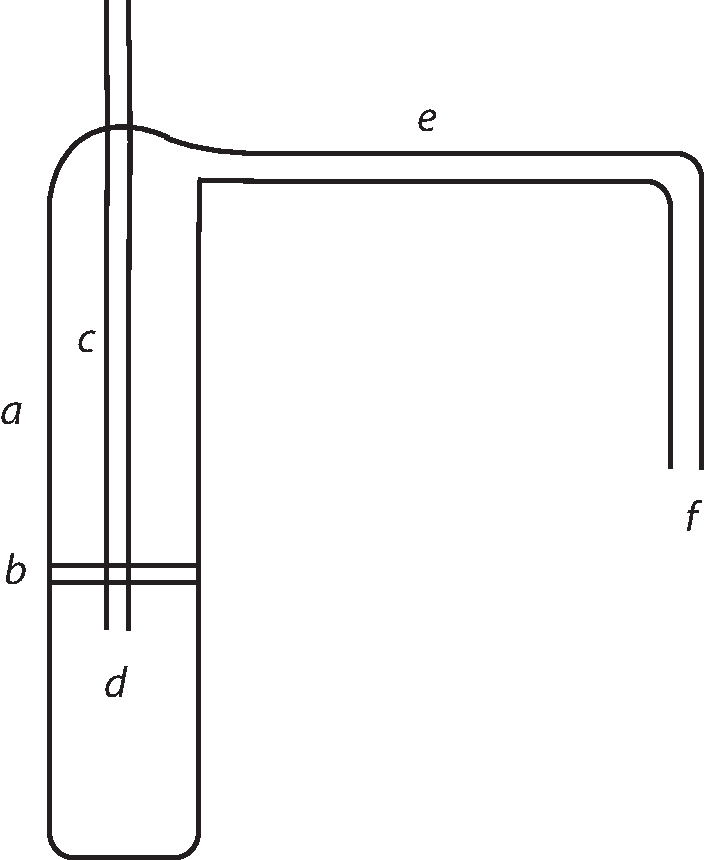
\includegraphics[width=0.4\textwidth]{images/LH35_14_2_95v}
                \\\textit{[Fig. 1]}
                        %\caption{Bildbeschreibung}
                       \end{center} 
                       \pstart   \edtext{\textso{Cap. 8.}}{\lemma{\textso{8.}}\Bfootnote{\textsc{O. v. Guericke}, \cite{00055}a.a.O., S.~81\textendash84.}} Vacuum Summum.  Ex vase \textit{a} aqua  repleto ad \textit{b} in quam  descendit Tubulus longus, sed  tenuis \textit{cd}  aqua plenus. Aerem extrahit\edlabel{gigni2} per \textit{ef} orificio \textit{f}  intrans in recipiens Magdeburgicum\protect\index{Sachverzeichnis}{Recipiens!Magdeburgicum}.  
                        %@ @ @ Dies ist eine Abstandszeile - fuer den Fall, dass mehrere figures hintereinander kommen, ohne dass dazwischen laengerer Text steht. Dies kann zu einer Fahlermeldung fuehren. @ @ @ \\
                     Ita enim  continuis suctionibus non aqua, sed aer omnis in  ea resuctus exit, et aqua penitus descendit ex \textit{cd}  usque ad \edtext{horizontem altitudinis aquae  circumfusae}{\lemma{horizontem}\Afootnote{ \textit{ (1) }\ ordinariae \textit{ (2) }\ altitudinis aquae  circumfusae \textit{ L}}} \textit{b}. Ita semper vacuum demonstrari \edtext{potest, inversa machinula,}{\lemma{potest,}\Afootnote{ \textit{ (1) }\ aere \textit{ (2) }\ inversa machinula, \textit{ L}}} ut \textit{cd} impleatur aqua,  et iterum erecta, ut tota aqua ex ea exeat. Et  vero subinde bullae oriebantur, sed \textit{e} inverso tubo  statim \edtext{versus}{\lemma{statim}\Afootnote{ \textit{ (1) }\ per majus \textit{ (2) }\ versus \textit{ L}}} \textit{ef} tenebant. Et ait semper  novas generatas successu temporis ejusmodi bullas  nisi magnitudine circiter, eversione Tubi \textit{cd} expellendas. (+ Hinc contra ipsum probatur nunquam intus  ostendi posse verum vacuum. Hinc aquam aere perfecte  purgare difficile: at contra Boylius\protect\index{Namensregister}{\textso{Boyle} (Boylius, Boyl., Boyl), Robert 1627\textendash 1691} et Hugenius\protect\index{Namensregister}{\textso{Huygens} (Hugenius, Vgenius, Hugens, Huguens), Christiaan 1629\textendash 1695}, purgare se  ajunt posse, at non diu. +) \textit{Si Machinula  impleatur cerevisia, ad dimidiam scilicet partem, ut ante  factum erat aqua, et postea extrahatur, tunc tota }\edtext{\textit{Cerevisia}}{\lemma{\textit{tota}}\Afootnote{ \textit{ (1) }\ \textit{aqua} \textit{ (2) }\ \textit{Cerevisia} \textit{ L}}}\textit{  in spumam redigitur seque ita elevat, ut partim in }\textit{siphonem}\protect\index{Sachverzeichnis}{sipho}\textit{ }\textit{e}\textit{ ascendat.} Si subito aperiatur aditus aeri externo, tunc  is tanta vi aquam ascendere facit in \textit{cd} ut pars \textit{e}  vi avellatur. Etiam machinula lente inflectenda est,  ut aqua in \textit{cd} intret, alioquin tanto impetu illabitur, ut duritiem lapidis referat, quo Tubi vitrei franguntur  et tunc externus aer per \textit{c} irrumpens in \textit{a} ipsum  quoque disrumpet. \textit{Cavendum quoque ne nimis vibretur machinula}\footnote{NB}\textit{  frangitur enim. Notatu hoc loco dignum est, quod aqua  e fistula minori }\textit{cd}\textit{ (quando scilicet machinula per aliquot  tempus inversa, ac sic fistula aqua repleta steterit, posteaque  erigitur) non descendat, }\textit{\textso{etiamsi fistula 100 credo ulnas  alta esset.}}\textit{ Ratio haec est quod aqua in se ita consolidatur, et  conjungitur, ut nullo in loco velit initium sese disjungendi  vel rumpendi sumere, nisi machinula illidatur ad mensam  vel pavimentum tunc ob violentiam, et quidem cum fragore rumpit aliquo loco incerto quamvis cum maximo fistulae periculo. Idem facit \mercury \, bene lavatum, nec hoc in passu  quicquam facit aerei cylindri gravitas. Sicut autem cum  tempore hi liquores ita consolidantur, ut absque violentia diruptionem non patiantur, tamen fallit quando fistula plena per unum  alterumve diem conservatur erecta (omnes enim liquores praesertim quando pendent, uti hoc modo aqua in fistula effluvium  quoddam aereum emittunt, quod cum tempore in Tubi apice conglobatur et discrimen vel separationem partium vitri scilicet  et liquorum causatur) namque tunc aqua communiter insperato invenitur delapsa.}
                     \pend 